\section{System Design}
In this section we elaborate the underlying system design which is capable of processing 2.4 million messages per second. We emphasize three features of this design. Firstly between any two nodes there is a set of TCP connections (typically 20 connections)  to send messages. All processes share the same set of connections which we called the bridge. The advantage of this approach compared to having TCP connections per process is that it utilizes all available bandwidth even there is only one process per node. However since this is a common bridge now we have to send the receiving process id to dispatch the message, sending  process id to parse the message and sequence number to order messages. As we discuss later our experiments show that this approach perform several times better than the other systems despite the above overhead. Secondly we have implemented \textit{OutputStream} and \textit{InputStream} interfaces on top of java non blocking I/O API. Using these input and output streams we provide \textit{DataOutput} and \textit{DataInput} APIs to directly 
serialize message data to binary format without sending any metadata along the message. Finally except messages themselves, all the other objects used to serialize and parse the messages and parse the messages are not created at message processing time. All these objects are created when a process sends the first message and it is a one-time cost. Rest of this section further explains the design techniques we used to realize these concepts.
\subsection{Inter Process Communication}
Figure \ref{interprocess} shows the design involved in sending a message from one process to another. Lets assume there is a message at a client side process and that process wants to send this message to another process. First the client process sends this message to its \textit{ElementContainer}. \textit{ElementContainer} holds all the streams (this is an abstraction of a link in the process graph) to which this message needs to send and it push the message to all streams. Stream decides which node to send this message and passes the message along the target node details to \textit{ConnectionManager} which holds \textit{ClientConnection}s for each node. \textit{ConnectionManager} sends message to correct \textit{ClientConnection} using target node. \textit{ClientConnection} picks an available \textit{DataOutput} from its pool of \textit{DataOutputs} and invokes the serialize method of the message to send that to server side.

At the server side there is a set of \textit{ServerTask}s which reads receiving messages from a pool of \textit{DataInput} streams available in the \textit{ServerConnection} (we register these connections at the connections creating time). Once a \textit{ServerTask} receives a binary message, it creates the event using the sending process id to identify the event type. Then it passes this message to the \textit{WorkerContainer} which holds all processes. Finally \textit{WorkerContainer} dispatches this message to correct process using receiving process id. Message ordering happens at the process level if required. This illustrates how we have shared a pool of TCP connections among processes and next we show how we have implemented \textit{OutputStream} and \textit{InputStream} with non blocking I/O API without  creating objects dynamically.
\begin{figure}[!tii]
        \centering
        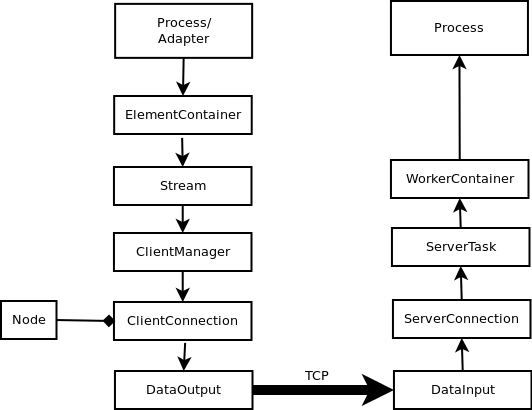
\includegraphics[width=3.0in]{interprocess.png}
        \caption{Communication between two Process}
        \label{interprocess}
\end{figure}
\subsection{Client Side}
Figure \ref{client} shows how we have implemented \textit{OutputStream} interface using our \textit{DataWriter}. \textit{DataWriter} contains a \textit{ByteBuffer}. When a higher layer method writes data to \textit{DataOuput}, \textit{DataWriter} puts those bytes to its byte buffer. When a selection event occurs, \textit{Datawriter} writes its byte buffer to underline \textit{SocketChannel}. This way only one byte buffer is used as an intermediary to create an output stream with non blocking I/O API.
\begin{figure}[!t]
        \centering
        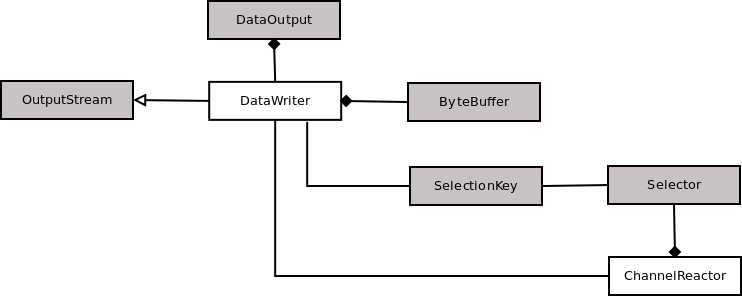
\includegraphics[width=3.0in]{client.png}
        \caption{OutputStream Implementation}
        \label{client}
\end{figure}
\subsection{Server Side}
Figure \ref{server} shows how we have implemented \textit{InputStream} interface using our \textit{DataReader}. Similar to client side, \textit{DataReader} has a \textit{ByteBuffer}. When a selection event occurs \textit{DataReader} inputs bytes from the \textit{SocketChannel} to its byte buffer. When a \textit{ServerTask} reads data through \textit{DataInput}, it reads data from the byte buffer and passes to higher layer. In this way we have implemented an input stream with non blocking I/O API.
\begin{figure}[!t]
        \centering
        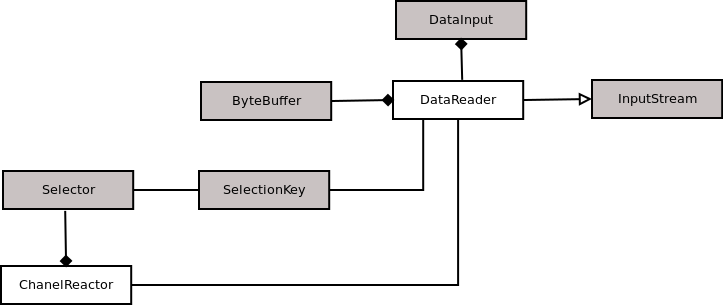
\includegraphics[width=3.0in]{server.png}
        \caption{InputStream Implementation}
        \label{server}
\end{figure}
